
Gracias a la infraestructura desarrollada dentro del experimento \textbf{CMS}, los equipos de análisis de física de altas energías ahora pueden preservar fácilmente su código de análisis en formatos de contenedores Linux, de modo que pueda usarse con fines de reinterpretación, con ellos viene incluido como una receta, el orden exacto en que las diversas tareas de un análisis deben llevarse a cabo y el conocimiento de cómo usarlo exactamente para poder extraer nueva ciencia.

Entre las herramientas más básicas y robusta de la biblioteca desarrollada por el \CERN ~es el programa orientado a objetos \ROOT, este fue originalmente fue diseñado para el análisis de datos de física de partículas y contiene varias características específicas de este campo. Este proporciona todas las funcionalidades necesarias para manejar el procesamiento de grandes datos, el análisis estadístico, la visualización y el almacenamiento. Está escrito principalmente en $\mathbf{C^{++}}$ pero integrado con otros lenguajes como $\mathbf{Python}$ y $\mathbf{R}$, es la base también de muchos de sus sistemas, conteniendo las librerías necesarias para su ejecución.

El proyecto \textbf{RECAST} (\textbf{R}equest \textbf{E}fficiency \textbf{C}omputation for \textbf{A}lternative \textbf{S}ignal \textbf{T}heo\-ries) combina la motivación científica para un poderoso programa de reinterpretación en el \LHC ~ con las capacidades técnicas que ofrecen los lenguajes de flujo de trabajo y los entornos de software. Los principales grupos de búsqueda dentro de la colaboración \LHC~ ahora requieren que se conserven nuevos análisis utilizando estas nuevas herramientas, de modo que cuando los teóricos proponen un nuevo modelo de física, la colaboración puede reutilizar estos análisis archivados para derivar una primera evaluación a través de la reinterpretación. También se espera que los análisis conservados se usen en una ola de estudios de resumen planificados una vez que se finalicen los análisis de datos de la segunda ejecución del \LHC, entre ellos los modelos supersimétricos, %denominado \MSSM ~ fenomenológico y 
de esta forma permitir una evaluación detallada del estado de la supersimetría más allá del alcance más estrecho de los modelos individuales. 

%La implementación de estas herramientas y su completo control son habilidades necesarias para incursionar en la investigación de altas energías, de aquí que se precise profundizar en ellas.


\subsection{Implementando \ROOT}\label{C_root}
Como ya se trato anteriormente \ROOT \footnote{Página del Proyecto: \href{https://root.cern.ch}{https://root.cern.ch}}~ es un ``\textit{framework}'' para el procesamiento de datos, nacido en el \CERN, dedicado principalmente para la investigación sobre física de altas energías. Todos los días, miles de físicos utilizan aplicaciones \ROOT ~para analizar sus datos o realizar simulaciones, entre sus utilidades encontramos:
\begin{itemize_f}
\item \textbf{Guardar datos:} compactación en forma binaria comprimida en un archivo de extensión $\mathbf{*.root}$, siendo archivos autodescriptivos, por lo que facilita obtener información sobre los modelos utilizados para describirlos. Su característica principal es ser un contenedor de datos llamado árbol, con sus subestructuras ramas (``\textit{branch}'') y hojas (``\textit{leave}''). Un árbol puede verse como una ventana deslizante a los datos sin procesar, tal como se almacenan en un archivo. Los datos de la siguiente entrada en el archivo se pueden recuperar avanzando el índice en el árbol. Esto evita los problemas de asignación de memoria asociados con la creación de objetos y permite que el árbol actúe como un contenedor liviano mientras se maneja el almacenamiento.

\item \textbf{Acceso a los datos:} se accede a los datos guardados en uno o varios archivos \ROOT ~ desde la web o sistemas de entrega de archivos a gran escala. Los árboles \ROOT ~ distribuidos en varios archivos se pueden encadenar y acceder como un objeto único, lo que permite bucles sobre grandes cantidades de datos.

\item \textbf{Mina de datos:} posee potentes herramientas matemáticas y estadísticas para operar con sus datos, todo sobre $\mathbf{C^{++}}$, pŕeparado para el procesamiento en paralelo cuando se requiera la manipulación de los mismos. Permite la generación de cualquier distribución estadística y modelados, logrando simular sistemas complejos.

\item \textbf{Gráfica resultados:} los datos se pueden mostrar con histogramas, diagramas de dispersión, funciones de ajuste ya integradas como herramientas en su biblioteca.

\item \textbf{Ejecución interactiva o creación de aplicaciones:} Puede usar el intérprete Cling $\mathbf{C}^{++}$ para sus sesiones interactivas y para escribir macros, o puede compilar su programa para que se ejecute a toda velocidad, siempre dando la posibilidad de crear una interfaz gráfica de usuario.
\end{itemize_f}

Hay muchas herramientas creadas a partir de \ROOT, entre ellas se pueden destacar el generador \MC ~ (\textbf{M}onte \textbf{C}arlos) $\mathbf{Madgraph}$, y entre las herramientas interactivas a $\mathbf{EVE}$.


%\begin{figure}[ht!]
%    \centering
%    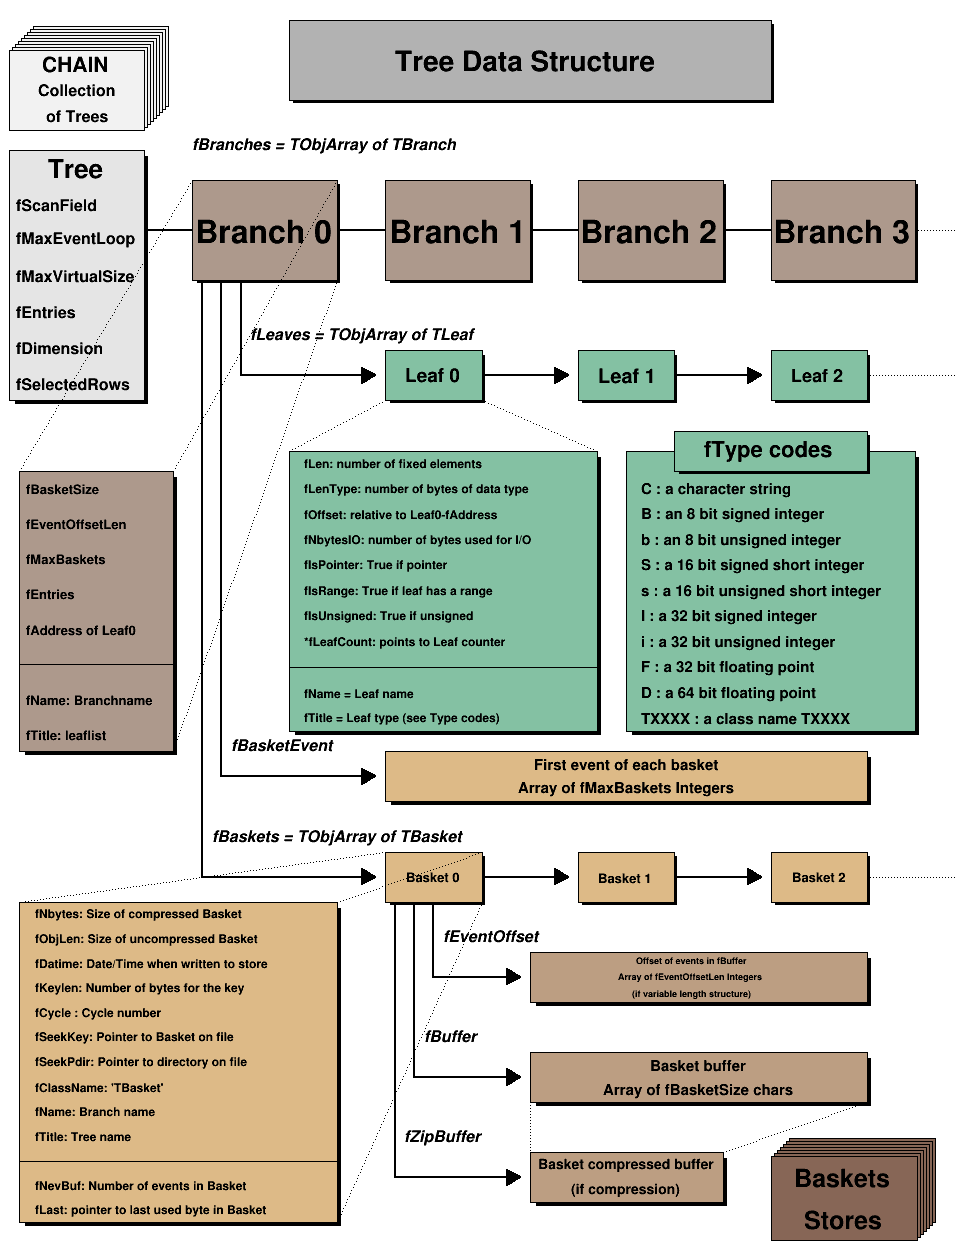
\includegraphics[width=0.84\textwidth]{Analisis_y_Resultados/imagenes/trees_root.png}
%    \caption{Estructura de los datos en forma de árbol.}
%    \label{fig:trees_root}
%\end{figure}

\subsection{Generador Monte Carlos con $\mathbf{Madgraph5}$}\label{C_madgraph}

Las colisiones de alta energía entre partículas elementales normalmente dan lugar a estados finales complejos, con grandes multiplicidades de hadrones, leptones, fotones y neutrinos. La relación entre estos estados finales y la descripción física subyacente no es simple, ya que no se posee una comprensión completa de la física a implementar y cualquier enfoque analítico se vuelve intratable por las grandes multiplicidades.

La forma de abordar este problemática es generando eventos completos por los métodos de \MC, la complejidad se domina mediante una subdivisión del problema completo en un conjunto de tareas separadas más simples, simulando todos los aspectos principales de los eventos: selección de procesos duros, la radiación de estado inicial y final, los restos de haces, la fragmentación, las desintegraciones, el cálculo de secciones transversales y su coincidencia con generadores de eventos, etc. Esto resulta en eventos que deben ser directamente comparables con los observables experimentalmentes y de esta forma programas pueden usarse para extraer la física de las comparaciones con los datos existentes, o para estudiar la física en experimentos futuristas.

Con el objetivo de refundir un análisis \LHC ~siendo una de sus herramientas mas importantes desarrollada por el proyecto y la solución a los problemas anteriormente planteado tenemos a $\mathbf{MadGraph5\_aMC}$ \citep{alwall_automated_2014} siendo un ``\textit{framework}'' que tiene como objetivo proporcionar todos los elementos necesarios para la fenomenología del \ME ~ y extensiones, permitiendo el uso de una variedad de herramientas relevantes para generación, manipulación y análisis de eventos. 

%Toda la información con respecto a su instalación y configuración se puede encontrar en su página oficial: \url{https://twiki.cern.ch/twiki/bin/view/CMSPublic/MadgraphTutorial}. 

La salida del mismo son archivos $\mathbf{*.lhe}$ o \textbf{LHEF} (\textbf{L}es \textbf{H}ouches \textbf{E}vent \textbf{F}ile), estos datos son los que obtenemos de un generador \MC (\textbf{M}onte \textbf{C}arlos) como $\mathbf{MadGraph5\_aMC}$. Esta salida contiene varios parámetros cinemáticos de todas las partículas involucradas en los procesos junto con la descripción de procesos simulados, parámetros de modelo y condiciones de ejecución. El análisis con \textbf{LHEF} se realiza para comprender varias propiedades cinemáticas básicas de la muestra de \MC ~ producida. Las variables cinemáticas asociadas con diferentes partículas del evento se pueden obtener utilizando este método.


El principal conjunto de herramientas que componen la herramienta $\mathbf{MadGraph5\_aMC}$, o a las que puede ser integrada son: 
$\mathbf{Delphes}$ (\cite{de_favereau_delphes_2014-1}), 
$\mathbf{MadAnalysis4}$ y $\mathbf{MadAnalysis5}$ \citep{conte_madanalysis_2013}, 
$\mathbf{ExRootAnalysis}$, $\mathbf{Golem95}$ \citep{binoth_precise_2008}, 
$\mathbf{QCDLoop}$ %\citep{ellis_scalar_2008}
, 
$\mathbf{maddm}$ %\citep{wang_novel_2018}
, 
$\mathbf{maddump}$ %\citep{buonocore_event_2019}
, 
$\mathbf{pythia8}$ \citep{pythia8}, 
$\mathbf{lhapdf5}$ y 
$\mathbf{lhapdf6}$ \citep{buckley_lhapdf6_2015}, 
$\mathbf{collier}$ \citep{denner_collier_2017}, 
$\mathbf{hepmc}$, 
$\mathbf{mg5amc\_py8\_interface}$, 
$\mathbf{ninja}$ %\citep{hirschi_tensor_2016, peraro_ninja_2014, mastrolia_integrand_2012}
, 
$\mathbf{oneloop}$ %\citep{van_hameren_oneloop_2011}
. 
Su implementación se hace necesaria para estudios de partículas, dada su versatilidad, aunque sea una herramienta de altas exigencias en conocimiento de programación y trabajo en el sistema Linux. 

Para uso futuro como parte de esta investigación se profundizará en las herramientas $\mathbf{pythia8}$ y $\mathbf{Delphes}$, estás a pesar de poderse ejecutar de forma independiente pueden ser integradas con facilidad dentro del programa de $\mathbf{Madgraph}$ y de esta manera planificar la receta de nuestro proceso a reconstruir.



\subsection{Hadronización con $\mathbf{pythia8}$}\label{C_pythia8}

El programa $\mathbf{pythia8}$ \citep{sjostrand_introduction_2015} es una herramienta estándar para la generación de colisiones de alta energía con mas de 35 a\~nos de desarrollo y actualización, este comprende un conjunto coherente de modelos físicos para la evolución de un proceso difícil de pocos cuerpos a un estado final multihadrónico complejo. Contiene una biblioteca de procesos y modelos complejos para los estados inicial y final del \textit{parton showers} \citep{nagy_what_2018}, múltiples interacciones de \textit{parton-parton}, \textit{beam remnants}, \textit{tring fragmentation} y \textit{article decays}. También tiene un conjunto de utilidades e interfaces para programas externos.  

Las versiones anteriores se escribieron en $\mathbf{Fortran}$, aunque ha sido completamente reescritura $\mathbf{C^{++}}$. Su versión mas actual es una opción atractiva para los estudios de física del \LHC ~ pero el programa también se utiliza para una multitud de otros estudios fenomenológicos o experimentales.

Las principales tareas realizadas por el programa incluyen la exploración de las consecuencias experimentales de los modelos teóricos, el desarrollo de estrategias de búsqueda, la interpretación de datos experimentales y el estudio del rendimiento del detector. De este modo, abarca toda la vida útil de un experimento, desde los primeros conceptos de diseño para el detector hasta la presentación final de los datos. %En este caso particular, sin embargo, \textbf{Pythia} solo se usa para hadronizar la muestra de \textbf{MC} producida por MadGraph.

\subsubsection{Limitaciones}

Los modelos de física incorporados en $\mathbf{pythia8}$ se centran en colisiones de partículas de alta energía que tienen energías de \textbf{C}entro de \textbf{M}asa (\textbf{CM}) mayores de $10 ~ \mathbf{GeV}$, correspondientes a una energía de haz fijo de protón-protón $pp \geq 50 ~ \mathbf{GeV}$. Esta limitación se debe a la aproximación de un continuo de estados finales permitidos que se utilizan en varios lugares de $\mathbf{pythia8}$, especialmente para los cálculos de la sección transversal hadron-hadron, total y diferencial, y como base para el modelo de fragmentación de cuerdas. Con energías inferiores a $10 ~ \mathbf{GeV}$, ingresamos a la región de resonancia hadrónica, donde estas aproximaciones se rompen, y por lo tanto los resultados producidos por $\mathbf{pythia8}$ no serían confiables. El límite de $10 ~ \mathbf{GeV}$ se elige como una escala típica; para la aniquilación positrón-electrón ($e+$ $e-$) sería posible ir algo más bajo, mientras que para las colisiones $pp$ los modelos no son particularmente confiables cerca del límite inferior.

En el extremo opuesto, solo es conocido pruebas explícitas de la física de $\mathbf{pythia8}$ que modela hasta energías \textbf{CM} de aproximadamente $100 ~ \mathbf{TeV}$, que corresponde a una energía de haz de objetivo fijo de $pp~\leq~10^{10} ~ \mathbf{GeV}$. Además, el programa solo funciona con colisiones hadron-hadron o lepton-lepton, las instalaciones internas para manejar las colisiones protón-núcleo o núcleo-núcleo no están previstas en absoluto. Entre los hadrones incluidos se encuentra el antiprotón, antineutrón, el pión y, como caso especial, el Pomeron. Todavía no hay ninguna disposición para las colisiones de leptones-hadrones o para los haces de fotones entrantes.

La producción de partículas salientes es en vacío y la simulación de la interacción de las partículas producidas con el material detector no está incluida en $\mathbf{pythia8}$. Las interfaces con los códigos de simulación de detectores externos pueden ser escritas directamente por el usuario o realizadas a través de la interfaz $\mathbf{HepMC}$.

\subsubsection{Procesos incluidos}

Una gran cantidad de procesos están disponibles internamente, y aún más a través de interfaces para programas externos. Las adiciones internas recientes incluyen varios escenarios para la física de Hidden Valley, procesos adicionales que involucran dimensiones adicionales, más procesos supersimétricos (\textbf{SUSY}), manejo extendido de R-hadrones y más estados de charmonium y bottomonium. En la correspondiente última versión 8.2, los siguientes procesos están disponibles internamente:

\begin{itemize_f}
\item \textbf{Los procesos de Electrodébiles o \textbf{EW} (\textbf{E}lectro\textbf{W}eak):} incluyen la producción rápida de fotones, la producción individual de $\gamma/Z$ y $W\pm$, así como la producción de pares de bosones débiles con correlaciones de fermiones completas.%, además de los procesos de colisión de fotones del tipo $\gamma \gamma \rightarrow ff$.
\item \textbf{Producción de fermiones de cuarta generación:} a través de interacciones electro-débiles o fuertes.
\item \textbf{Los procesos de Higgs:} incluyen la producción del bosón Higgs del \ME, así como los múltiples bosones Higgs de un modelo genérico de dos dobletes de Higgs o \textbf{2HDM}(Two-\textbf{H}iggs-\textbf{D}oublet \textbf{M}odel). %También es posible modificar la correlación angular del decaimiento de Higgs $h \rightarrow V V \rightarrow 4f$ debido a acoplamientos anómalos de $hV V$. 
La implementación interna de \SUSY ~ también utiliza la implementación $\mathbf{2HDM}$ para su sector Higgs.
\item \textbf{Los procesos \SUSY:} incluyen la producción de pares de partículas \SUSY, así como la producción resonante de squarks a través de la paridad \textit{R} que viola la interacción \textbf{UDD}. Las interferencias electro débil se han tenido en cuenta cuando sean relevantes. Se puede hacer que tanto los squarks como los gluinos formen R-hadrones de larga vida, que posteriormente se descomponen. En el medio, es posible cambiar el contenido de sabor ordinario de los hadrones R, mediante interacciones (implementadas por el usuario) con el material del detector.
\item \textbf{Los procesos de calibre de bosones :} se incluyen la producción de un $Z'$ (con interferencia completa de $\gamma^*/Z/Z'$), un $W^{'\pm}$ y un bosón de calibre de acoplamiento horizontal (entre generaciones) $R^0$.
\item[-] \textbf{Otros Procesos :} Los procesos \textbf{QCD}, procesos simétricos de izquierda a derecha, producción de leptoquark, procesos de composición, procesos de Hidden Valley, procesos extradimensionales, producción Top, Onia.
\end{itemize_f}





\subsection{Simulando el detector con $\mathbf{Delphes 3}$}\label{C_delphes}



Este simula la respuesta de un detector compuesto por un rastreador interno (The silicon Tracker), calorímetros electromagnéticos y de hadrones (\textbf{ECAL} y \textbf{HCAL}) y un sistema detector de muones (ver referencia \cite{de_favereau_Delphes_2014}). Todos están organizados concéntricamente con una simetría cilíndrica alrededor del eje del haz. El usuario puede especificar el volumen activo del detector, la segmentación del calorímetro y la intensidad del campo magnético uniforme (Fig. \ref{Delphes}). Cada subdetector tiene una respuesta específica, como se describe a continuación.

\begin{figure}[!t]
    \centering
    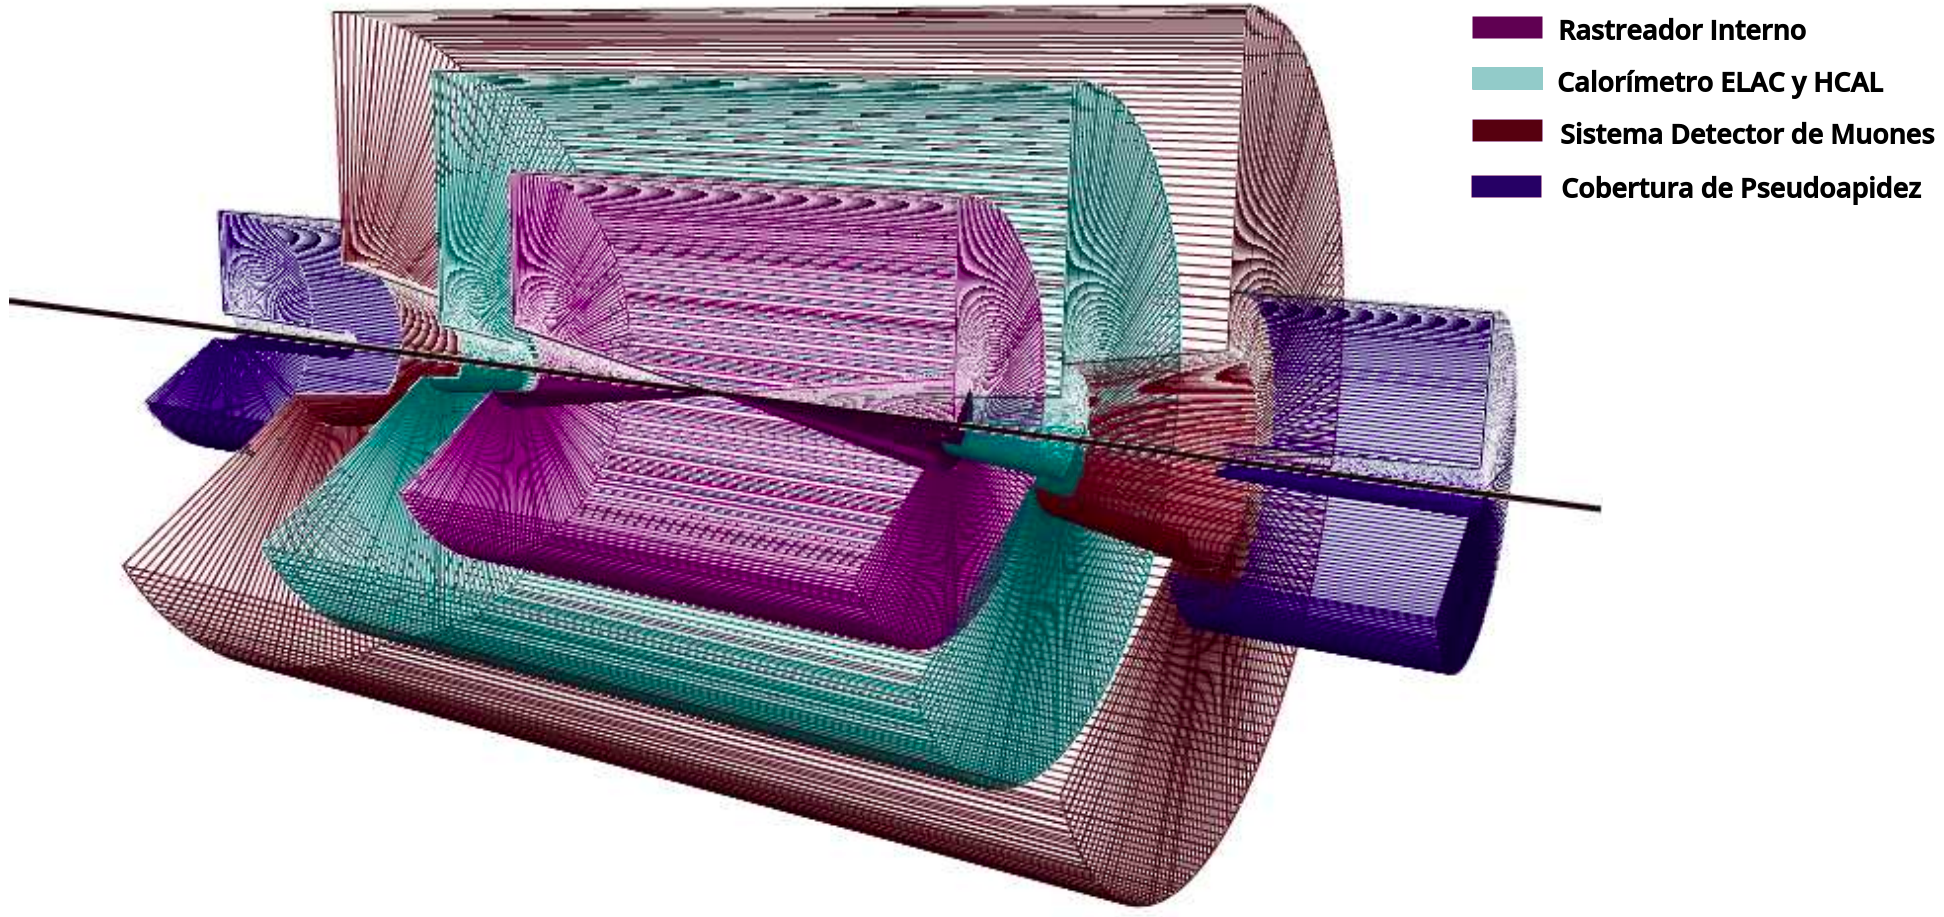
\includegraphics[width=.95\textwidth]{Analisis_y_Resultados/imagenes/delphes.png}
    \caption[Perfil de diseño básico de la geometría del detector genérico asumido en  \textbf{Delphes}.]{Perfil de diseño básico de la geometría del detector genérico asumido en  $\mathbf{Delphes}$.\footnotemark}
    \label{Delphes}
\end{figure}

\footnotetext{Adaptado del artículo de origen \cite{alwall_automated_2014}}

En $\mathbf{Delphes}$, la reconstrucción e identificación de objetos se basa en una serie de aproximaciones para acelerar sensiblemente el procedimiento y mantener una buena precisión. 

Los muones que se origina en la interacción, tiene cierta probabilidad de ser reconstruido, según la parametrización de eficiencia definida por el usuario. Esta probabilidad se desvanece fuera de la aceptación del rastreador, y para momentos de muón por debajo de algún umbral para rechazar partículas en bucle. El momento final del muón se obtiene mediante una mancha gaussiana del vector inicial de 4 momentos. La resolución es parametrizada en función de $p_T$ y $\eta$ implementada por el usuario.

El ``\textit{framework}'' $\mathbf{Delphes}$ permite el acceso a datos de diferentes formatos de archivo ($\mathbf{Pro}\-\mathbf{MC}$, $\mathbf{HEPMC}$, $\mathbf{STDHEP}$ y $\mathbf{LHEF}$). Los archivos de eventos provenientes de generadores externos \MC ~ son procesados primero por un lector, este convierte partículas estables en una colección de objetos universales, para luego ser procesada por una serie de módulos que comienzan con el módulo de fusión acumulada y terminan con el módulo de buscador de objetos único. Finalmente,  $\mathbf{Delphes}$ permite al usuario almacenar y analizar eventos en un formato de árbol raíz al ejecutar  $\mathbf{DelphesHepMC}$ tomando un archivo de configuración $\mathbf{*.tcl}$(``\textit{Delphes card}'') y realizando la simulación del detector en el archivo $\mathbf{*.hepmc}$. La información sobre varios objetos \textbf{MC} (partículas) y objetos reconstruidos (jets, partículas reconstruidas), estas se guardan en un archivo $\mathbf{*.root}$ en forma de árboles (``trees'')  \textbf{Delphes}, el archivo de salida $\mathbf{*.root}$ se puede abrir usando el mismo programa \ROOT.


%El aislamiento de un electrón, muón o fotón se realiza si la actividad en sus proximidades es lo suficientemente pequeña. Un objeto aislado tiene una pequeña probabilidad de originarse en un jet. Existen varias definiciones posibles para una variable de aislamiento, dependiendo del nivel particular de rechazo de señal a fondo que el analizador desea lograr. En  \textbf{Delphes} se opto por uno simple, muy adecuado para experimentos con colisionadores de hadrones. Una definición alternativa, más adecuada para los experimentos, basada en variables esféricas, aunque aún no se ha implementado en  \textbf{Delphes}, puede derivarse fácilmente de la presente. Además, la modularidad del marco permite al usuario otras definiciones, más adecuadas para diferentes experimentos o requisitos de análisis, o simplemente para no aplicar ningún criterio de aislamiento en los objetos finales.

















%
%
%La simulación de los distintos procesos físicos y la respuesta del detector a los mismos es necesaria para poder optimizar y estimar el desempeño de los diferentes análisis. Además, permite que las estrategias utilizadas en la identificación de partículas puedan ser desarrolladas con anterioridad a la toma de datos y las eficiencias de los algoritmos pueden ser puestos a prueba. La preparación de las búsquedas de nueva física necesitan una simulación detallada del detector para estimar su potencial de descubrimiento y para desarrollar métodos óptimos para medir las propiedades de las partículas.
%
%Es fundamental un correcto entendimiento de los procesos de señal y de fondo para poder distinguir entre ambos. Una vez que los datos de colisiones reales están disponibles, los datos simulados también resultan necesarios para poder encontrar desviaciones del \ME.
%La estructura de los eventos de colisiones de altas energías son realmente complejos y no predecibles de primeros principios. Los generadores de eventos permiten separar el problema en varios pasos más simples, algunos de los cuales pueden ser descriptos por primeros principios, y otros necesitan ser basados en modelos apropiados con parámetros ajustados a los datos. Un aspecto central de los generadores es que proveen una descripción del estado final para poder construir cualquier observable y compararlos con los datos de colisiones reales.
%
%
%
%
%
%
%
%
%
%
